\section{Methods}
\begin{figure*}
  \centering
  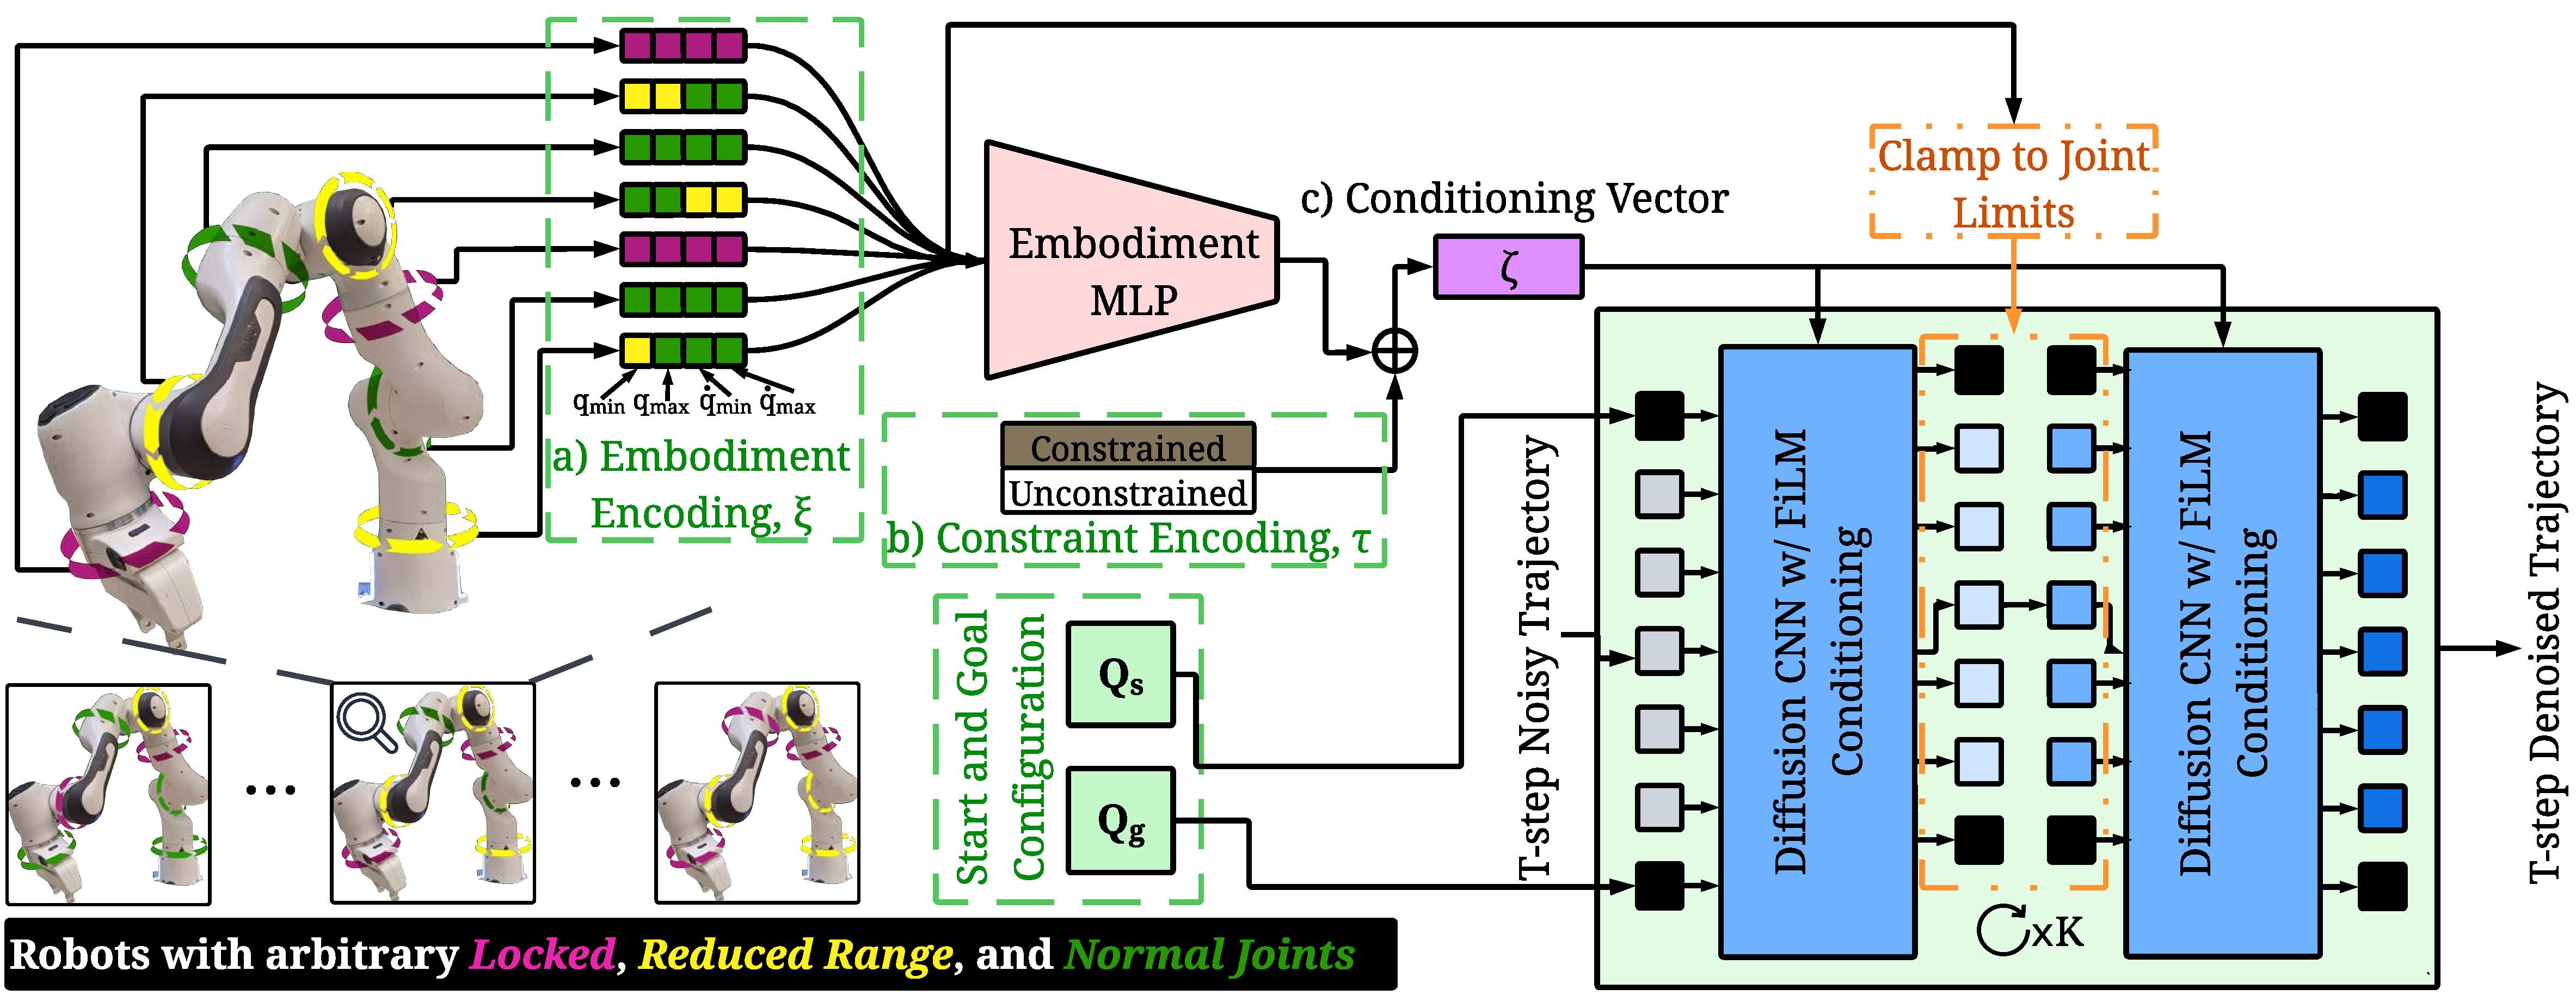
\includegraphics[width=\textwidth]{figures/block_diagram.pdf}
  \caption{Overview of DEFT. a) joint-level embodiment constraints are encoded into a structured representation capturing failure constrained joint position and velocity limits. This embodiment encoding is processed by a multilayer perceptron (MLP) and used to condition the diffusion model. b) Task-specific constraints (e.g. unconstrained or constrained) are represented as one-hot vectors and concatenated with the embodiment encoding to constrained the generative process. 
  Given these conditioning signals and start-goal joint configurations, the model generates feasible joint-space trajectories adapted explicitly to both the robot's degraded embodiment and task requirements. At each step of the denoising process the predicted joint values are clamped to the failure-induced robot joint limits. \vspace{-12pt}}
  \label{fig:system-diagram}
\end{figure*}
% \gm{Basically for the methods we need to describe only our contribution: diffusion for failure recovery, conditioning on embodiment, and conditioning on primitive, and inpainting (hardcoding but don't say this) the joint limits. We need to make sure this supports the narrative of 'diffusion rocks at failure recovery and we needed to add conditioning to close the sim to real gap'}

% \gm{We need: 1) an algorithm block on the diffusion approach, 2) plain english descriptions of \textbf{all} math, 3) remove unconstrained and constrained definitions}

% \gm{Finally, we need to write this methods section with reproducibility in mind. For another experienced PhD student, if they take this methods section, can they create our approach from scratch?}


% Our aim is to make robots fail-active by generating functional and feasible trajectories even in the event of joint-level failures.

% We frame this as a trajectory generation problem conditional on failure embodiment and task constraint. Each unique failure defines a new embodiment of the robot, and each task constraint (e.g., \texttt{unconstrained} or \texttt{constrained}) induces a distinct trajectory distribution. 
Our goal is fail-active manipulation: generate functional, feasible trajectories under joint-level failures. We pose this as conditional trajectory generation given the failure-induced embodiment and the task constraint. Each failure specifies a new embodiment of the robot, and each constraint (e.g., \texttt{unconstrained} vs. \texttt{constrained} motion) induces a distinct trajectory distribution. Given the start and goal joint configurations  the policy $\pi$ infers a future sequence of joint states over a fixed number of steps $T$. Unlike prior work that assumes a fixed set of failure configurations to control over, our method adapts online. It learns both the control behavior and the allowable motions from the current failure condition and the task constraint.
Our formulation enables zero shot trajectory generation across diverse embodiments and task conditions. For example, when a shoulder joint becomes unusable, the robot can switch from lifting to pushing an object without task specific retraining or policy switching.

\subsection{DEFT}
Inspired by recent advances in diffusion policies~\cite{chi2023diffusion}, we develop DEFT for an $N$-degrees of freedom robot to synthesize joint-space trajectories. Formally, the policy is defined as:
\begin{equation}
\pi(Q_{s,g}| \xi, \tau) \rightarrow \{\textbf{q}_{1:T}, \dot{\textbf{q}}_{1:T}\}
\end{equation}

The policy is conditioned on a vector $\xi \in \mathbb{R}^{4N}$ that encodes joint-level embodiment constraints imposed by the failure condition, and on a task constraint represented by a one-hot encoded vector $\tau$, as shown in \cref{fig:system-diagram}.

Given a ground-truth trajectory $\mathbf{x}$ and a diffusion time step, we first add Gaussian noise $\mathcal{N}(\mathbf{0}, \mathbf{I})$ to obtain a corrupted trajectory. We then inpaint the start and goal joint positions, $Q_{s,g} = [{(\textbf{q}_s, \dot{\textbf{q}}_s), (\textbf{q}_g, \dot{\textbf{q}}_g)}], q \in \mathbb{R}^N$, so endpoints remain exact. We proceed by clamping the entire noisy trajectory to the joint angle and velocity limits specified by the failure embedding $\xi = [\mathbf{e}_q, \mathbf{e}_{\dot{q}}] \in \mathbb{R}^{4N}$, ensuring feasibility under the current embodiment. Next, we form a conditioning vector, $\zeta = [\xi, \tau]^\top $,  by encoding the failure embedding with a small MLP and concatenating the resulting features to the task constraint token. The denoiser (UNet) receives the clamped, inpainted trajectory together with the time step and conditioning vector, and predicts a denoised trajectory $\hat{\mathbf{x}}$, denoising for $K=25$ steps as it showed no change in trajectory quality while having a inference speed improvement compared to \cite{chi2023diffusion}. Finally, we hard-enforce constraint adherence by clamping the prediction to the same limits and re-inpaint the endpoints, returning the denoised, feasible trajectory.


\subsection{Conditioning Approaches}
% \begin{algorithm}[t]
% \caption{Constraint-Aware Diffusion Step}
% \label{alg:diffusion}
% \KwIn{Ground-truth trajectory $\mathbf{x}$, timestep $t$, failure embedding $\mathbf{f}$, primitive encoding $\mathbf{p}$}
% \KwOut{Denoised trajectory $\hat{\mathbf{x}}$}
% Sample noise $\boldsymbol{\epsilon} \sim \mathcal{N}(0, I)$\;
% Compute noisy input: $\tilde{\mathbf{x}}_t = \sqrt{\alpha_t} \cdot \mathbf{x} + \sqrt{1 - \alpha_t} \cdot \boldsymbol{\epsilon}$\;
% \textbf{Inpaint} start and goal: $\tilde{\mathbf{x}}_t[\text{start/goal}] \leftarrow \mathbf{x}[\text{start/goal}]$\;
% \textbf{Clamp} $\tilde{\mathbf{x}}_t$ to limits specified by $\mathbf{f}$\;
% Fuse failure and primitive encodings: $\mathbf{c} \leftarrow \text{MLP}_f(\mathbf{f}) \, \| \, \text{MLP}_p(\mathbf{p})$\;
% Predict denoised trajectory: $\hat{\mathbf{x}} = \text{Unet}(\tilde{\mathbf{x}}_t, t, \mathbf{c})$\;
% \textbf{Clamp} output $\hat{\mathbf{x}}$ to limits in $\mathbf{f}$\;
% \textbf{Inpaint} start and goal: $\hat{\mathbf{x}}[\text{start/goal}] \leftarrow \mathbf{x}[\text{start/goal}]$\;
% \Return{$\hat{\mathbf{x}}$}
% \end{algorithm}
% Uses your existing \usepackage{algorithm} and \usepackage{algorithmic}
% \begin{algorithm}[t]
% \caption{\textit{DEFT}}
% \label{alg:diffusion}
% \begin{algorithmic}[1]
% \REQUIRE Denoising Steps $K$; Failure embedding $\mathbf{\xi}$; Primitive encoding $\mathbf{\tau}$
% \ENSURE Denoised trajectory $\hat{\mathbf{x}}$
% \STATE Sample noisy trajectory $\tilde{\mathbf{x}} \sim \mathcal{N}(\mathbf{0}, \mathbf{I})$
% % \STATE Compute noisy input: $\tilde{\mathbf{x}}_t \gets \sqrt{\alpha_t}\,\mathbf{x} + \sqrt{1 - \alpha_t}\,\boldsymbol{\epsilon}$
% \FORALL{$k\in K$}
%     \STATE Inpaint start and goal: $\tilde{\mathbf{x}}_t[\mathrm{start/goal}] \leftarrow  Q_{s,g} $
%     \STATE Clamp $\tilde{\mathbf{x}}_t$ to limits specified by $\mathbf{\xi}$
%     \STATE Fuse encodings: $\zeta \gets \mathrm{MLP}_\xi(\mathbf{\xi}) \,\|\, \mathbf{\tau}$
%     \STATE Predict denoised trajectory: $\hat{\mathbf{x}} \gets \mathrm{UNet}(\tilde{\mathbf{x}}_t,\, t,\, \zeta)$
%     \STATE Clamp output $\hat{\mathbf{x}}$ to limits in $\xi$
%     \STATE Inpaint start and goal: $\hat{\mathbf{x}}[\mathrm{start/goal}] \leftarrow  Q_{s,g} $
% \ENDFOR
% \RETURN $\hat{\mathbf{x}}$
% \end{algorithmic}
% \end{algorithm}

\begin{algorithm}[t]
\caption{DEFT}
\label{alg:diffusion}
\LinesNumbered % Adds line numbers
\KwIn{Denoising Steps $K$; Failure embedding $\mathbf{\xi}$; Primitive encoding $\mathbf{\tau}$}
\KwOut{Denoised trajectory $\hat{\mathbf{x}}$}

Sample noisy trajectory $\tilde{\mathbf{x}} \sim \mathcal{N}(\mathbf{0}, \mathbf{I})$\;

\ForEach{$k \in K$}{
    Inpaint start and goal: $\tilde{\mathbf{x}}_t[\mathrm{start/goal}] \leftarrow Q_{s,g}$\;
    Clamp $\tilde{\mathbf{x}}_t$ to limits specified by $\mathbf{\xi}$\;
    Fuse encodings: $\zeta \gets \mathrm{MLP}_\xi(\mathbf{\xi}) \,\|\, \mathbf{\tau}$\;
    Predict denoised trajectory: $\hat{\mathbf{x}} \gets \mathrm{UNet}(\tilde{\mathbf{x}}_t,\, t,\, \zeta)$\;
    Clamp output $\hat{\mathbf{x}}$ to limits in $\xi$\;
    Inpaint start and goal: $\hat{\mathbf{x}}[\mathrm{start/goal}] \leftarrow Q_{s,g}$\;
}
\Return{$\hat{\mathbf{x}}$}
\end{algorithm}

\subsubsection{Embodiment Conditioning}
To inform the model of the robot's failure constrained embodiment, we use an embodiment encoding vector $\xi$ to condition the diffusion model. We model joint-level failures as per-joint constraints on the robot's actuation capabilities. Each failure embodiment is represented as $\xi = [\mathbf{e}_q, \mathbf{e}_{\dot{q}}] \in \mathbb{R}^{4N}$, with $\mathbf{e}_{q,j} = [q_j^{\min}, q_j^{\max}]^\top$ and $\mathbf{e}_{\dot{q},j} = [\dot{q}_j^{\min}, \dot{q}_j^{\max}]^\top$ for all $j \in \{1,\dots,N\}$ such that $\mathbf{0} \in \mathbf{e}_{\dot{q},j}$\footnote{$\mathbf{0}$ must be in $\mathbf{e}_{\dot{q},j}$ to ensure a stable equilibrium point exists~\cite{blanchard_differential_2011}.}.  
 Failures reshape the robot’s feasible configuration space and task-space reachability and exist in a continuous space, allowing $\xi$ to capture a wide spectrum of degradation severities, as shown in \cref{fig:system-diagram}. Let $\{\mathbf{q}_t\}_{t=1}^T$ denote a trajectory over $T$ steps, where $\mathbf{q}_t \in \mathbb{R}^N$ is the joint configuration at time $t$, and $\dot{\mathbf{q}}_t$ its velocity. A configuration $\mathbf{q}_t$ satisfies the feasibility set $\mathcal{C}_t(\mathbf{q}_t,\xi)$ if:%
{\setlength{\abovedisplayskip}{6pt}\setlength{\belowdisplayskip}{6pt}\setlength{\abovedisplayshortskip}{4pt}\setlength{\belowdisplayshortskip}{4pt}%
\begin{equation}
\begin{aligned}
\small
  \mathcal{C}_t(\mathbf{q}_t,\xi)=\Big\{\mathbf{q}_t\in\mathbb{R}^N\ \Big|\ 
  q_{t,j}\in \mathbf{e}_{q,j},\ \dot{q}_{t,j}\in \mathbf{e}_{\dot{q},j}\ \\ \ \forall j\in\{1,\dots,N\}\Big\}.
\end{aligned}
\end{equation}}%
A trajectory is feasible if $\mathbf{q}_{1:T}\in\bigcap_{t=1}^T \mathcal{C}_t(\mathbf{q}_t,\xi)$, i.e. the joint trajectory for the time horizon $T$ should be within joint limits. We condition on failures structurally: the model learns to generate motion plans that obey the constraints.%
To integrate embodiment information into the generative process, we pass $\xi$ through an MLP to produce an embedding that modulates the diffusion model via FiLM. To ensure that the trajectory connects the desired start and goal states we apply start–goal inpainting, fixing $(\mathbf{q}_s,\mathbf{q}_g)$ in the input trajectory. This anchors the trajectory; without it, the stochastic denoiser may miss hard endpoint constraints. In addition, we clamp the trajectory to the limits during both training and inference: conditioning guides the model toward feasibility but does not guarantee it, so clamping enforces satisfaction of the joint constraints.


\subsubsection{Constraint Conditioning}  
We further condition the model on discrete task constraints using a one-hot encoding vector, $\tau$. Let $\tau \in \{0,1\}^K$ be a one-hot vector with exactly one nonzero entry, such that  
\[
\sum_{k=1}^{K} \tau_k = 1 
\quad \text{and} \quad 
\tau_k \in \{0,1\} \ \forall k.
\]  
We concatenate $\tau$ with $\xi$ to form the conditioning vector $\zeta = [\xi, \tau]^\top$, which is injected via FiLM.  

These constraints are not explicitly enforced during inference but must be learned implicitly through the conditioning signal. The constraint encoding also informs the model of task-imposed end effector constraints, which it otherwise would not know while operating in joint space.



% The primitive vector $\tau$ is processed through concatenated with the failure embedding. The combined representation is injected through FiLM into the diffusion model. This allows the model to distinguish contact regimes and synthesize motion accordingly. Primitive selection is externally provided at inference and does not require recognition.

\subsection{Data Generation Approaches}
\label{sec:data_generation}
% \begin{wrapfigure}{r}{0.55\textwidth}
% \vspace{-10pt}
% \begin{minipage}{0.55\textwidth}
% \begin{algorithm}[H]\small
% \caption{\small Trajectory Generation with Failure Conditioning (Constrained \& Unconstrained)}
% \label{alg:traj_generation}
% \begin{algorithmic}[1]
% \REQUIRE Start-goal pairs $Q_{s,g}$, nominal joint limits $\mathbf{Q}, \dot{\mathbf{Q}}$, primitive encoding $\tau$
% \ENSURE Valid trajectories with associated failure-conditioned limits

% \FORALL{$(\mathbf{q}_{\text{s}}, \mathbf{q}_{\text{g}}) \in Q(s,g)$}
%     \IF{$\tau = \texttt{constrained}$}
%         \STATE $\mathbf{p}_{1:T} \gets \textsc{InterpolateEEPath}(\mathbf{q}_{\text{s}}, \mathbf{q}_{\text{g}})$
%         \STATE $\mathbf{q}_{1:T} \gets \textsc{SolveIKPath}(\mathbf{p}_{1:T})$
%     \ELSIF{$\tau = \texttt{unconstrained}$}
%         \STATE $\mathbf{q}_{1:T} \gets \textsc{RRTConnect}(\mathbf{q}_{\text{s}}, \mathbf{q}_{\text{g}})$
%     \ENDIF

%     \IF{$\textsc{IsValid}(\mathbf{q}_{1:T}, \tau)$}
%         \STATE $(\mathbf{q}, \dot{\mathbf{q}}) \gets \textsc{MinJerkOptimize}(\mathbf{q}_{1:T})$
%         \STATE $J_f \gets \textsc{SampleFailureJoints}()$
%         \STATE $f \gets \textsc{SampleFailureType}()$
%         \STATE $\xi\gets \textsc{ApplyFailures}(J_f, f, \mathbf{q}, \dot{\mathbf{q}}, \mathbf{Q}, \dot{\mathbf{Q}})$
%         \STATE $\textsc{StoreTrajectory}(\mathbf{q}, \dot{\mathbf{q}}, \xi, \tau)$
%     \ENDIF
% \ENDFOR
% \end{algorithmic}
% \end{algorithm}
\begin{algorithm}
\small
\caption{Trajectory Generation with Failure Conditioning (Constrained \& Unconstrained)}
\label{alg:traj_generation}
\LinesNumbered
\KwIn{Start-goal pairs $Q_{s,g}$, nominal joint limits $\mathbf{Q}, \dot{\mathbf{Q}}$, primitive encoding $\tau$}
\KwOut{Valid trajectories with associated failure-conditioned limits}

\ForEach{$(\mathbf{q}_{\text{s}}, \mathbf{q}_{\text{g}}) \in Q(s,g)$}{
    \eIf{$\tau = \texttt{constrained}$}{
        $\mathbf{p}_{1:T} \gets \textsc{InterpolateEEPath}(\mathbf{q}_{\text{s}}, \mathbf{q}_{\text{g}})$\;
        $\mathbf{q}_{1:T} \gets \textsc{SolveIKPath}(\mathbf{p}_{1:T})$\;
    }{
        \If{$\tau = \texttt{unconstrained}$}{
            $\mathbf{q}_{1:T} \gets \textsc{RRTConnect}(\mathbf{q}_{\text{s}}, \mathbf{q}_{\text{g}})$\;
        }
    }

    \If{$\textsc{IsValid}(\mathbf{q}_{1:T}, \tau)$}{
        $(\mathbf{q}, \dot{\mathbf{q}}) \gets \textsc{MinJerkOptimize}(\mathbf{q}_{1:T})$\;
        $J_f \gets \textsc{SampleFailureJoints}()$\;
        $f \gets \textsc{SampleFailureType}()$\;
        $\xi\gets \textsc{ApplyFailures}(J_f, f, \mathbf{q}, \dot{\mathbf{q}}, \mathbf{Q}, \dot{\mathbf{Q}})$\;
        $\textsc{StoreTrajectory}(\mathbf{q}, \dot{\mathbf{q}}, \xi, \tau)$\;
    }
}
\end{algorithm}

% \end{minipage}
% \vspace{-10pt}
% \end{wrapfigure}


We generate a dataset of failure-conditioned joint-space trajectories for two distinct task constraints: \texttt{constrained} and \texttt{unconstrained}. Each trajectory $\mathbf{q}_{1:T} \in \mathbb{R}^{T \times N}$ consists of $T$ joint configurations sampled at fixed intervals of $\Delta t$ seconds. These trajectories are used to train and evaluate our diffusion-based planning framework.
% \paragraph{Primitive Conditioning.}
% Each trajectory is labeled with a primitive $\tau \in \{\texttt{push}, \texttt{unconstrained}\}$ indicating the type of manipulation strategy. Primitives reflect differences in contact constraints and control authority, and are encoded as one-hot vectors provided as model inputs.

\paragraph{Start and Goal Sampling}
For unconstrained, start and goal configurations $(\mathbf{q}_\text{s}, \mathbf{q}_\text{g})$ are sampled over nominal joint limits and filtered for feasibility using self-collision checks and workspace bounds. For constrained, we instead filter for joint configurations that have planar end-effector poses $(p_\text{s}, p_\text{g})$ at a fixed $z$-height.

\paragraph{Trajectory Construction}
As shown in Algorithm \ref{alg:traj_generation}, Unconstrained trajectories are computed using an RRT-Connect joint-space planner with goal biasing. Constrained trajectories are generated by interpolating end-effector poses along a straight Cartesian path, then solving for each joint configuration using an optimization-based IK solver with pose consistency constraints. All trajectories are smoothed in time using minimum-jerk optimization to produce zero-velocity endpoints and continuous velocity profiles $(\dot{\mathbf{q}}_t)$.


\paragraph{Failure Condition Sampling}
To simulate embodiment degradation, we sample a structured failure vector $\xi$ per trajectory. We first select the number of affected joints, ranging from one to seven, using a modified exponential decay distribution. Assuming  single joint failures are the most common, we fix the probability of a single joint failing at exactly 50\%, while the remaining 50\% probability is distributed among multiple joint failures such that each additional joint failure is half as likely as the one before it. We then sample one of three failure types: joint angle range reduction, velocity limit reduction, or combination. Modified joint limits are computed from the trajectory’s observed values with added uniform noise margins. In particular, for angle range reduction, the joint's feasible position and velocity range are tightened to encompass the observed extrema with an added random buffer  $\epsilon $.

% which introduces additional randomness to the failure condition.

% The failure vector $\xi$ is passed through a multilayer perceptron to produce a compact embedding. This embedding encodes the robot’s per-joint physical limits relative to nominal values (Appendix~\ref{app:failures}). This learned representation is injected at each residual block of the U-Net via FiLM, providing per-channel modulation during the denoising process.

\paragraph{Task Validity Filtering}
For both constraints, only trajectories that obey the constraint-specific requirements are retained. For constrained motions, validity is determined by: 1) total change in end-effector alignment, 2) manipulability above a certain threshold, and 3) path efficiency measured as the length between the two points as compared to the arc length of the generated path. For unconstrained, we verify feasibility using manipulability and goal reachability checks.

% \paragraph{Parallelized Execution.}
% We deploy a hybrid multiprocessing architecture across 30 CPU cores. Each worker processes a batch of start-goal pairs, generates valid trajectories, and queues the results. A separate writer process asynchronously commits data to three preallocated HDF5 files storing trajectories, auxiliary metadata (e.g., arc length, duration), and per-joint failure matrices. Progress is tracked using a global counter and a centralized task monitor.



% \paragraph{Output Format.}
% The final dataset contains $N_\text{traj} = 336 \cdot N$ trajectories stored in:
% \begin{itemize}
%   \item \texttt{trajectories.hdf5}: $\mathbf{q}_{1:T}$, $\dot{\mathbf{q}}_{1:T}$, $\ddot{\mathbf{q}}_{1:T}$
%   \item \texttt{aux\_data.hdf5}: arc length, duration, time parameterization
%   \item \texttt{failure\_data.hdf5}: joint limit matrices and failure vectors
% \end{itemize}



% \subsection{Training Setup}
% \input{algorithms/training}
% We train the model using simulated data from the Franka Emika Panda. Unconstrained trajectories are generated using CuRobo; push and poke primitives are synthesized via differential inverse kinematics. All trajectories are normalized to $[-1,1]$ based on nominal joint limits.

% Training uses AdamW with a cosine schedule, batch size 256, and 500 epochs. We apply EMA upd

% Here, $(q, \dot{q})$ denote joint positions and velocities. The failure vector $\xi$ encodes joint-level constraints across position and velocity for each of the 7 joints, and the task primitive  These inputs condition the model to generate embodiment-aware, task-aligned trajectories.



% \subsection{Conditioning Approaches}
% \paragraph{Failures as Embodiment Constraints}
% We model joint-level failures as per-joint constraints on the robot's actuation capabilities. Each failure embodiment encoding is represented by a structured vector $\xi$, comprising per-joint limits on position and velocity. Specifically, for each joint $j \in \{1, \dots, 7\}$, we define motion ranges $[q_j^{\min}, q_j^{\max}]$ and symmetric velocity bounds $[-\dot{q}_j^{\max}, \dot{q}_j^{\max}]$ that reshape the robot’s feasible configuration space and task-space reachability. Failures exist in a continuous space, allowing $\xi$ to represent a wide spectrum of degradation severities rather than a fixed set of discrete failure modes. A trajectory $\{\mathbf{q}_t\}_{t=1}^T$ is valid under $\xi$ if, for all $t$, the positions and velocities satisfy:
% \begin{equation}
%     \mathcal{C}_t(\xi) = \left\{ \mathbf{q}_t \in \mathbb{R}^7 \;\middle|\;
%     q_j^{\min} \leq q_{t,j} \leq q_j^{\max},\;
%     |\dot{q}_{t,j}| \leq \dot{q}_j^{\max}
%     \;\;\forall j \in \{1, \dots, 7\} \right\}.
% \end{equation}
% The full trajectory must satisfy $\mathbf{q}_{1:T} \in \bigcap_{t=1}^T \mathcal{C}_t(\xi)$. Critically, we treat failures not as noise to overcome, but as structured conditioning on the embodiment: the model learns to generate motion plans that succeed \emph{because of} the constraints.

% To integrate embodiment information into the generative process, we pass $\xi$ through a multilayer perceptron (MLP) to produce a compact embedding, which modulates the diffusion model’s internal features via Feature-wise Linear Modulation (FiLM). This allows DEFT to adapt the denoising process dynamically to the specific constraints imposed by each failure condition.



% \paragraph{Task Conditioning via Primitives}
% We condition the model on the intended manipulation primitive using a discrete variable $\tau$ It is concatenated with the failure-conditioned embedding and injected into the model via FiLM layers at each residual block, enabling the network to synthesize trajectories that align with the constraints and affordances of the specified primitive.

% \paragraph{Unconstrained Primitive.}
% We define \textbf{Unconstrained} as a motion primitive corresponding to unconstrained manipulation, where the object is rigidly secured relative to the end-effector. The goal of Unconstrained is to move from an initial pose to a goal pose without requiring sustained environmental contact during the motion. No specific path shape or additional geometric constraint is imposed beyond start and goal satisfaction and feasibility under embodiment constraints.

% Unconstrained defines a minimally constrained motion primitive appropriate for grasped object relocation or end-effector repositioning. The valid set of trajectories is:

% \begin{equation}
% \mathcal{T}_\text{unconstrained} = \left\{ \mathbf{q}_{1:T} \;\middle|\;
% \mathbf{q}_1 = \mathbf{q}_\text{start},\;
% \mathbf{q}_T = \mathbf{q}_\text{goal},\;
% \mathbf{q}_{1:T} \in \mathcal{C}_{1:T}(\xi)
% \right\}
% \end{equation}
% \paragraph{Constrained Primitive.}
% We define \textbf{Constrained} as a motion primitive that describes planar, approximately straight-line movement with minimal orientation change. Unlike primitives that specify force or contact interaction, Constrained constrains only the geometric form of the motion. Specifically, it requires the end-effector to move within a fixed plane, remain near a straight path between start and goal, and maintain a consistent orientation throughout the trajectory.

% This primitive serves as a geometric substrate that can support a variety of constrained behaviors—such as pushing, pulling, or surface tracing—through additional contact or force constraints at the task level. Constrained is particularly useful for fail-active planning, where manipulation must proceed under embodiment constraints that restrict the robot's motion capabilities.

% \begin{equation}
% \mathcal{T}_\text{constrained} = \left\{ \mathbf{q}_{1:T} \;\middle|\;
% \forall t, \; \left( \mathbf{p}_t \in \mathcal{P}_\text{plane} \;\land\;
% \texttt{Deviation}(\mathbf{p}_t) \leq \epsilon_p \;\land\;
% \|\mathbf{R}_t - \mathbf{R}_\text{start}\|_F \leq \epsilon_R \;\land\;
% \mathbf{q}_t \in \mathcal{C}_t(\xi) \right)
% \right\}
% \end{equation}

% These primitive-specific constraints are never explicitly enforced during inference but must be learned implicitly through the conditioning signal. The one-hot primitive encoding $\tau$ provides the model with task context, allowing it to specialize its generation behavior to different manipulation strategies.